\documentclass{article}
\usepackage{graphicx} % Required for inserting images
\usepackage{float}
\usepackage{amsmath}

\title{Diet Diversity Econometric Methodology}
\author{Carl Dinkel}
\date{March 2026}

\begin{document}

\maketitle

\section{Introduction}

The econometric work presented here was done to analyze and test out the proposed dietary diversity score/index. To do this and ensure the index can be used in research such as 'Banking On Biodiversity', rich/poor households were compared as way to ground the measurement in welfare relevancy. 

\section{Data Preparation}

The analysis uses household survey data containing detailed modules on household composition, food consumption, and household assets.

The core datasets used are:

\begin{itemize}
\item \textbf{Household roster (Section 2)}: demographic characteristics of household members (sex, age).
\item \textbf{Food consumption module (Section 15B)}: quantities of food consumed during the previous 7 days.
\item \textbf{Presence module (Section 15A)}: number of individuals present in the household during the last week.
\item \textbf{Asset module (Section 14)}: household asset values used as a proxy for wealth.
\end{itemize}

All modules were merged using the household identifier $HHID$ as well as the person identifier $PID$.

\section{Construction of Food Consumption Quantities}

Food consumption was recorded in a variety of units (kg, liters, bundles, cups, etc.). To obtain comparable quantities, all observations were converted to kilograms of food consumed.

The conversion followed a three-step hierarchy:

\begin{enumerate}
\item \textbf{Exact conversion factors}  

Known unit-to-weight mappings (e.g. kg, grams, standard packages).

\item \textbf{Volume conversions}  

Units expressed in liters were converted to kilograms using food-specific density estimates.

\item \textbf{Approximate conversions}  

For ambiguous units (e.g. pieces or heaps), weights were approximated using typical food weights.
\end{enumerate}

Observations with unresolvable units were removed. This resulted in a consistent dataset containing food quantities measured in kilograms per household per week.

\section{Conversion to Caloric Intake}

Food quantities were converted to caloric values using a food composition table derived from FAO nutritional data.

For each food item:

\[
Calories_{hg} = Quantity^{kg}_{hg} \times kcal\_per\_kg_g
\]

where $h$ denotes the household and $g$ denotes the food item.

Food items were then grouped into EAT-Lancet food categories:

\begin{itemize}
\item starchy staples
\item pulses and nuts
\item fats
\item dairy
\item meat, fish, and eggs
\item fruits
\item vegetables
\item sugar
\end{itemize}

Non-nutritional categories such as salt, beverages, tobacco, and prepared food were excluded from the analysis.

\section{Household Caloric Shares}

For each household, calories were aggregated to obtain total weekly caloric intake:

\[
TotalCalories_h = \sum_g Calories_{hg}
\]

The caloric share of each food group was then calculated as:

\[
s_{hg} = \frac{Calories_{hg}}{TotalCalories_h}
\]

These shares describe the composition of the household diet independently of total calorie consumption.

\section{Household Demographic Adjustment}

Households differ in size and demographic composition. To account for this, household members were converted into adult-equivalent units (AE) using age- and sex-specific caloric requirements.

The adult equivalent weight of individual $i$ was defined as:

\[
AE_i = \frac{CalorieRequirement_i}{2500}
\]

where 2500 kcal represents the reference caloric requirement of an adult male.

Household adult equivalents were calculated as:

\[
AE_h^{roster} = \sum_i AE_i
\]

To account for temporary visitors and absences, the adult equivalent measure was adjusted using the number of individuals present in the household during the past 7 days:

\[
AE_h^{adj} = AE_h^{roster} \times 
\frac{N_h^{present,7d}}{N_h^{roster}}
\]

This adjustment ensures that caloric consumption is attributed to the individuals who actually consumed the food.

\section{Construction of the EAT-Lancet Diet Index}

Diet quality was evaluated relative to the EAT-Lancet reference diet. For each food group $g$, the recommended caloric share $t_g$ was defined based on the EAT-Lancet guidelines.

Deviation from the recommended diet was measured as:

\[
d_{hg} =
\begin{cases}
\max(0, s_{hg} - t_g) & \text{for overconsumed groups} \\
\max(0, t_g - s_{hg}) & \text{for underconsumed groups}
\end{cases}
\]

Overconsumption was penalized for:

\begin{itemize}
\item starchy staples
\item fats
\item sugar
\end{itemize}

Underconsumption was penalized for:

\begin{itemize}
\item pulses and nuts
\item fruits
\item vegetables
\item animal foods
\end{itemize}

These deviations were squared and weighted to reflect the nutritional importance of different food groups:

\[
I_h^{raw} = \sum_g w_g \cdot d_{hg}^2
\]

The weights assign higher penalties to deviations in nutritionally important groups such as fruits, vegetables, pulses, and sugar.

\section{Index Normalization}

The raw deviation index was normalized to lie between 0 and 1:

\[
EAT_h = 1 - \frac{I_h^{raw}}{P_{99}(I^{raw})}
\]

where $P_{99}(I^{raw})$ denotes the 99th percentile of the raw index distribution.

This normalization reduces the influence of extreme outliers while ensuring that:

\begin{itemize}
\item $EAT = 1$ indicates diets closest to the EAT-Lancet recommendations
\item $EAT = 0$ indicates diets with the largest deviations.
\end{itemize}

\section{Wealth Classification}

Households were classified into wealth groups based on the total value of household assets.

Asset values were log-transformed to account for strong skewness:

\[
Wealth_h = \log(AssetValue_h + 1)
\]

\begin{figure}[H]
    \centering
    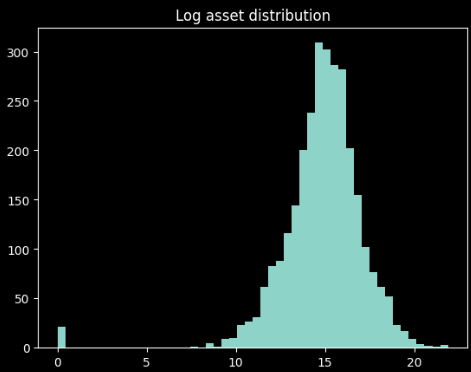
\includegraphics[width=0.72\textwidth]{distribution.png}
    \caption{Distribution of log-transformed household asset values. The figure illustrates the approximately bell-shaped distribution obtained after transforming raw asset values using $\log(AssetValue_h + 1)$. This transformation reduces skewness and improves the comparability of households across wealth quantiles.}
    \label{fig:asset_distribution}
\end{figure}


Households were then divided into wealth quintiles, with the bottom 20\% defined as poor households and the top 20\% defined as rich households.

\section{Comparative Analysis}

Diet quality was compared between poor and rich households using:

\begin{enumerate}
\item Mean EAT index values
\item Differences in caloric shares of food groups
\item Deviations from EAT-Lancet dietary targets
\end{enumerate}

Visualizations were used to illustrate how household diets diverge from recommended nutritional patterns across wealth groups.

Figure \ref{fig:eat_bar} presents the average weighted EAT-Lancet index for the poorest and richest household quintiles.

\begin{figure}[H]
    \centering
    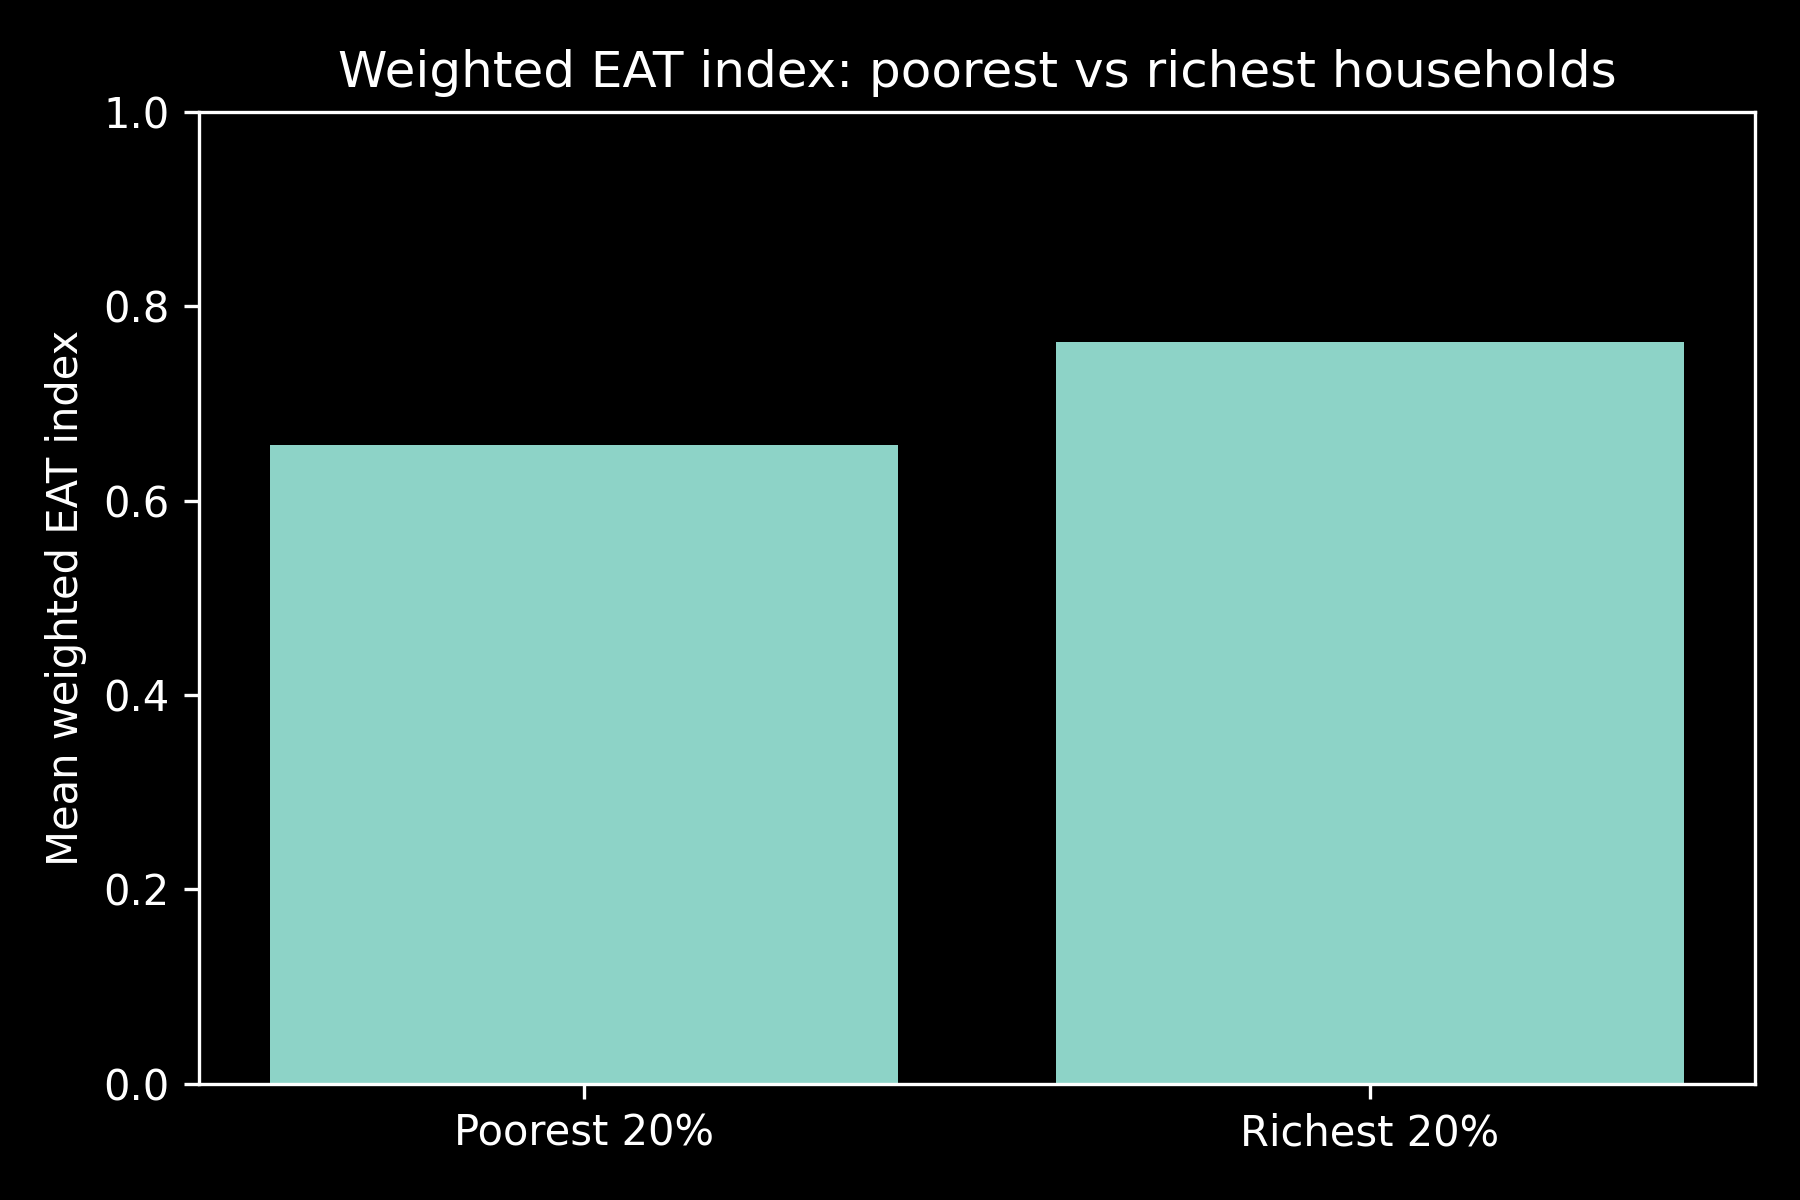
\includegraphics[width=0.72\textwidth]{eat_index_poor_vs_rich_bar.png}
    \caption{Mean weighted EAT-Lancet index for the poorest and richest household quintiles. Higher values indicate closer adherence to the EAT-Lancet reference diet. The figure shows that richer households exhibit, on average, higher diet quality than poorer households.}
    \label{fig:eat_bar}
\end{figure}

Figure \ref{fig:eat_bar} presents the average weighted EAT-Lancet index for the poorest and richest household quintiles.

\begin{figure}[H]
    \centering
    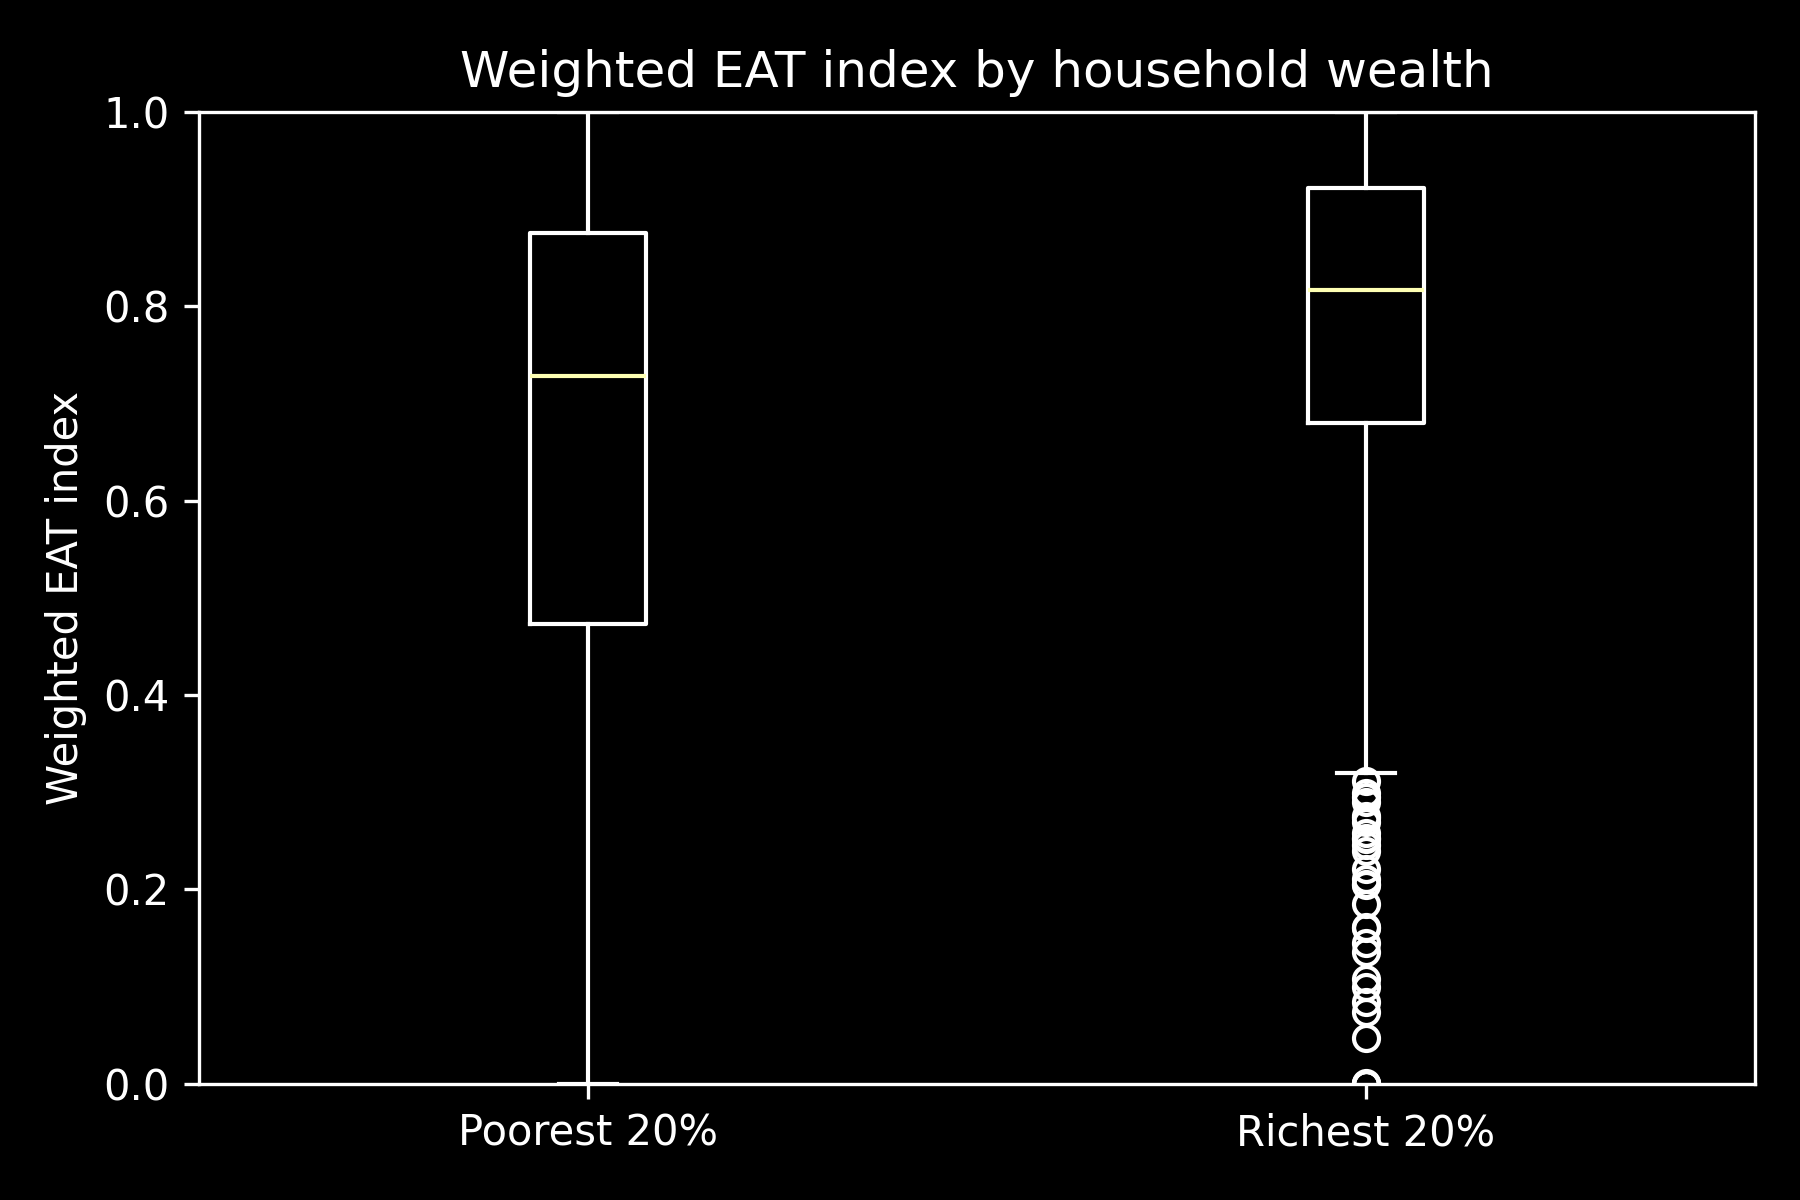
\includegraphics[width=0.72\textwidth]{eat_index_boxplot_poor_vs_rich.png}
    \caption{Distribution of the weighted EAT-Lancet index by household wealth group. The boxplots show that the richest quintile has a higher median index and a more favorable overall distribution than the poorest quintile, although substantial within-group heterogeneity remains.}
    \label{fig:eat_box}
\end{figure}

Figure \ref{fig:eat_hist} further illustrates the distribution of the weighted EAT-Lancet index across wealth groups.

\begin{figure}[H]
    \centering
    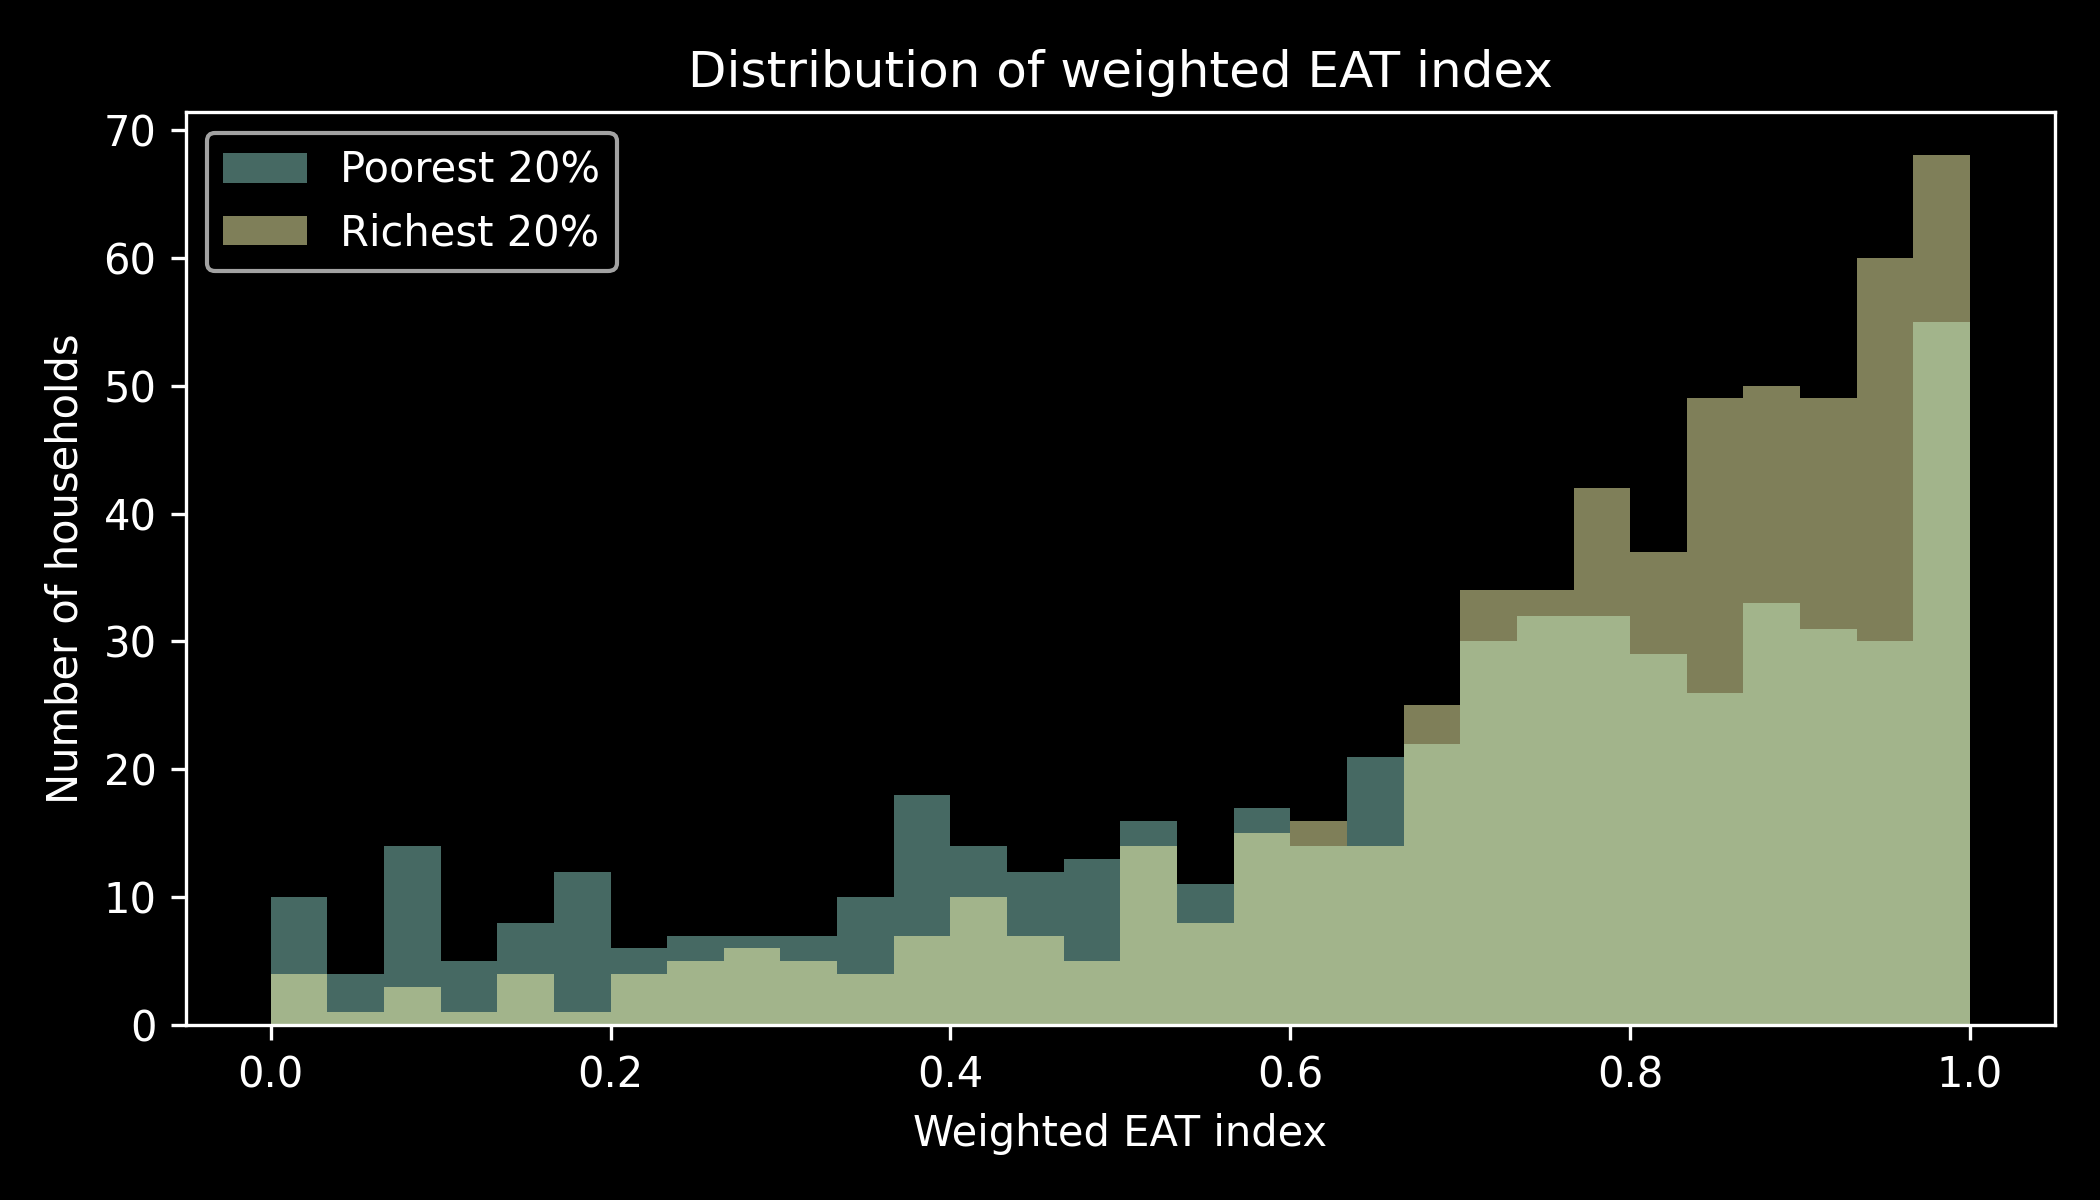
\includegraphics[width=0.78\textwidth]{eat_index_distribution_poor_vs_rich.png}
    \caption{Distribution of the weighted EAT-Lancet index for the poorest and richest household quintiles. The histogram suggests that the distribution for richer households is shifted toward higher values, consistent with greater dietary adherence relative to the EAT-Lancet reference diet.}
    \label{fig:eat_hist}
\end{figure}

To identify which food groups drive differences in the weighted EAT-Lancet index, Figure \ref{fig:eat_deviation} plots deviations in calorie shares from the reference diet for the poorest and richest household quintiles.

\begin{figure}[H]
    \centering
    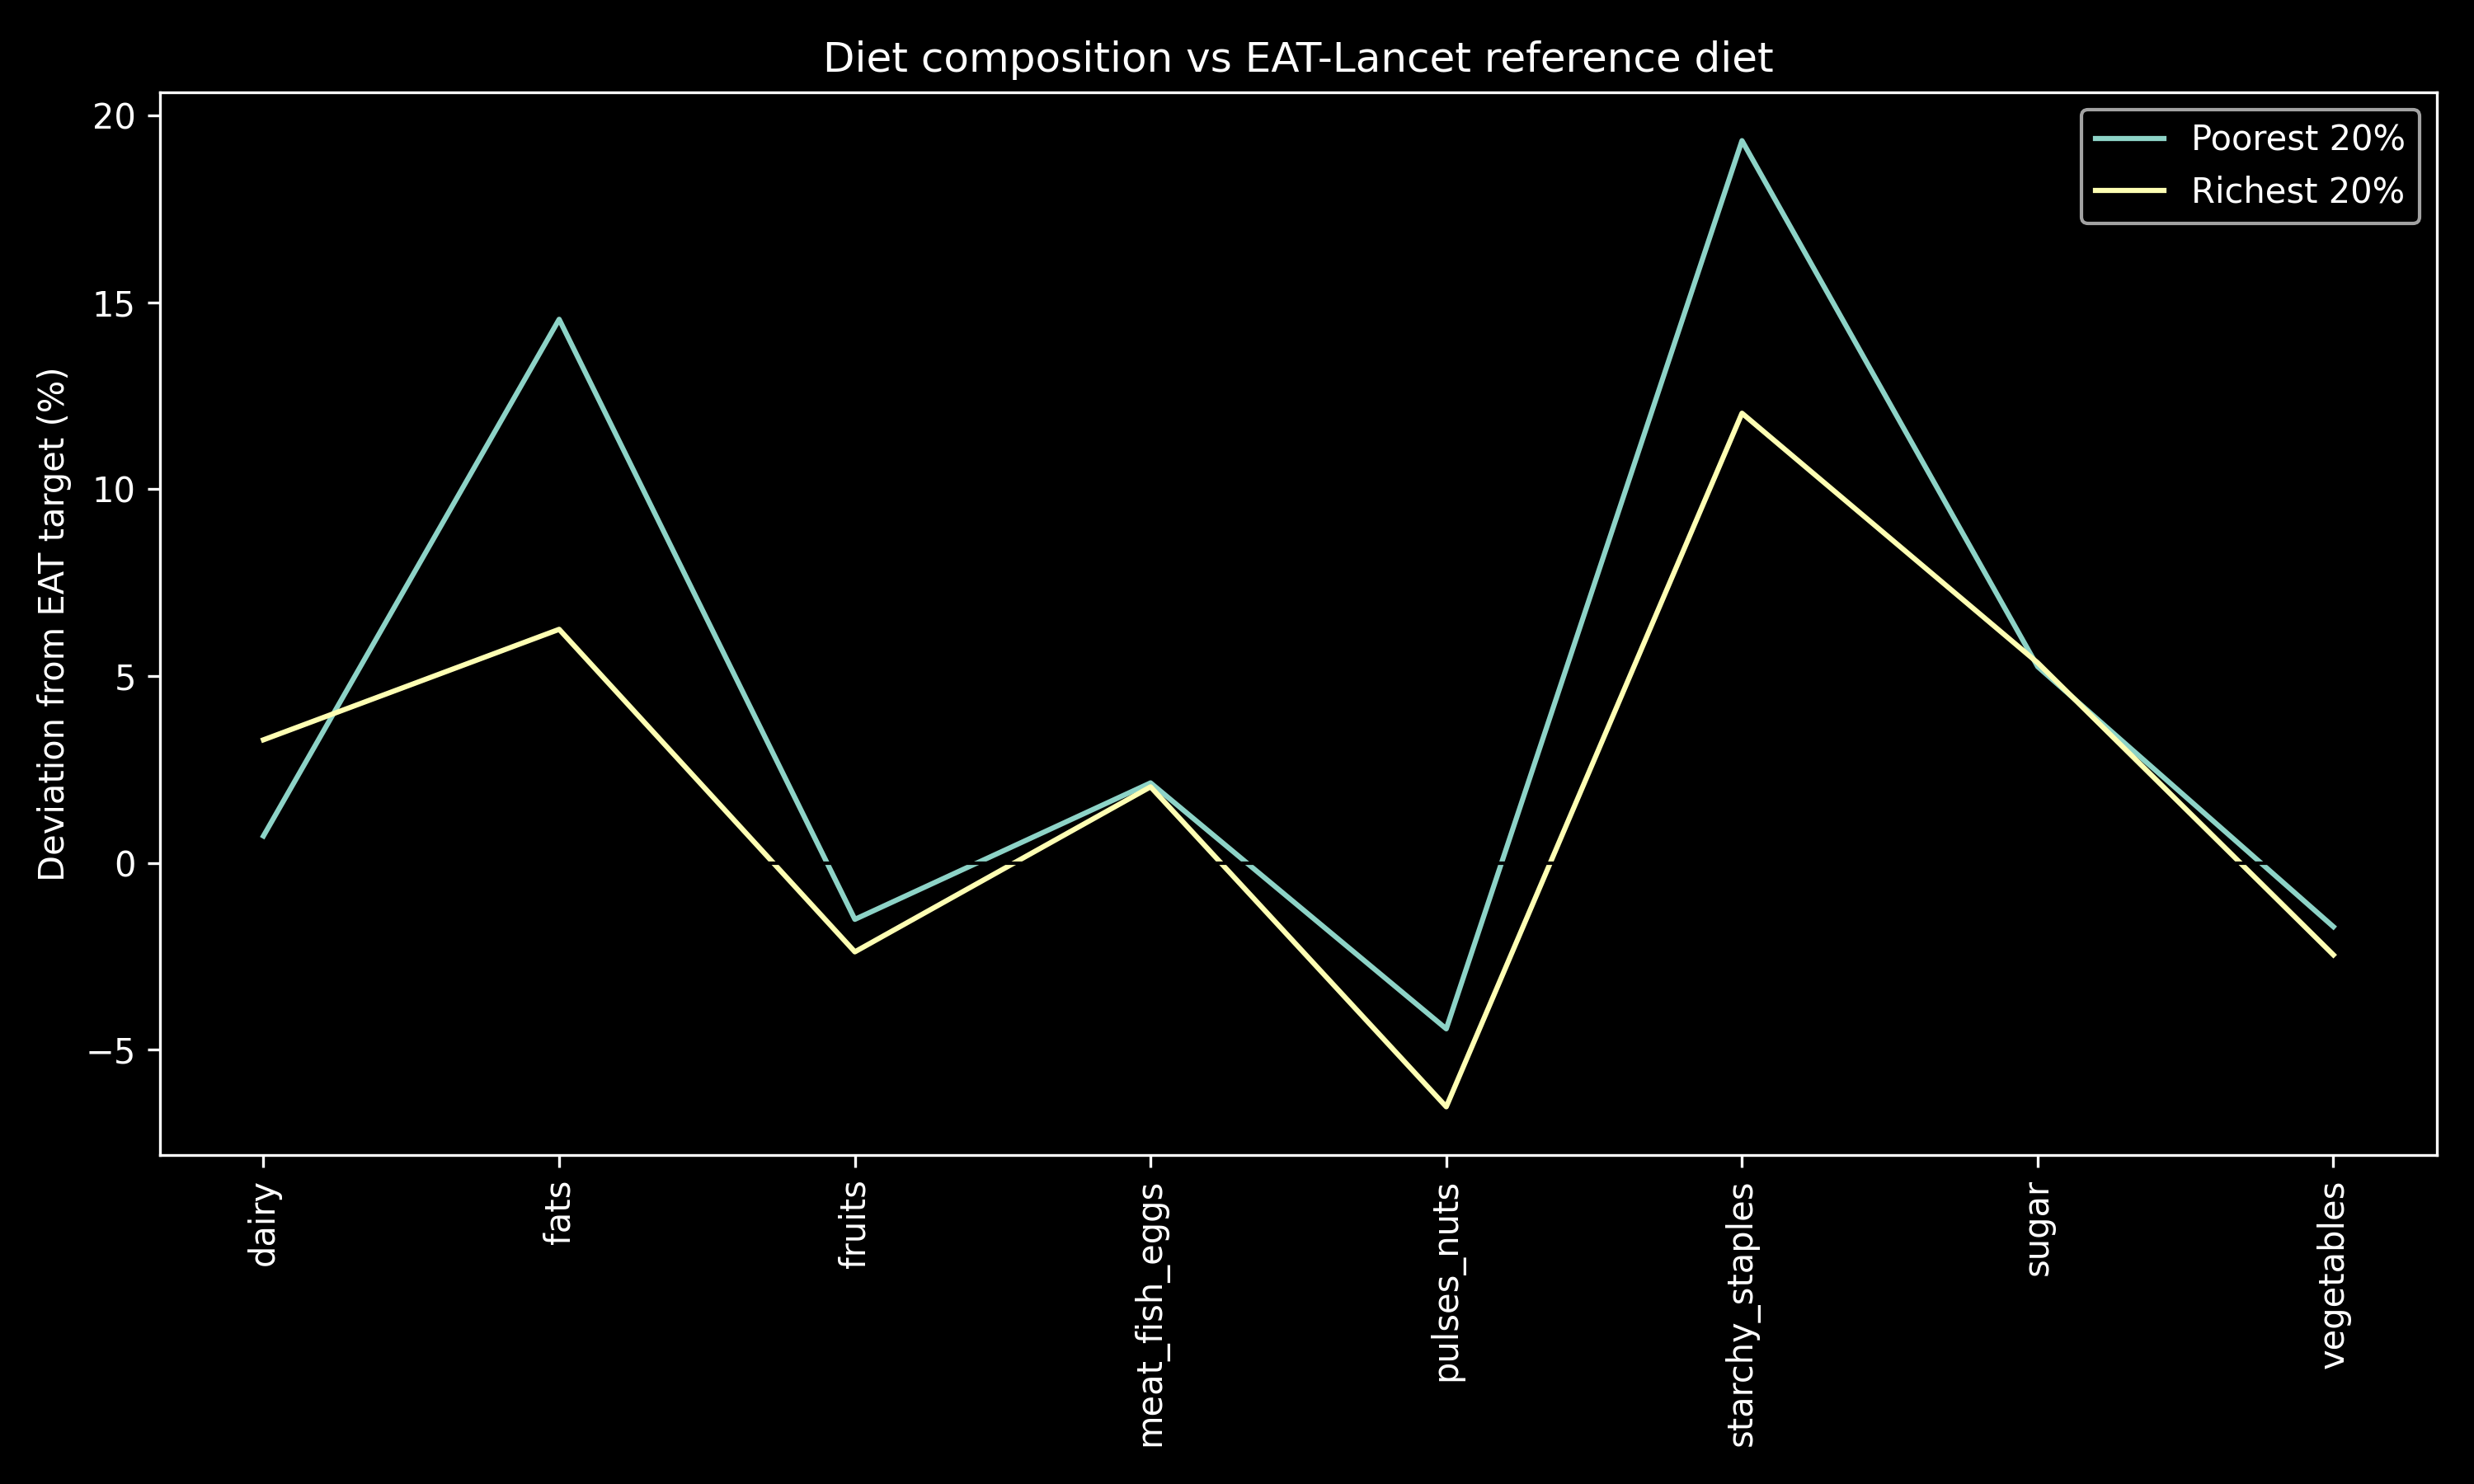
\includegraphics[width=0.82\textwidth]{eat_lancet_deviation_plot.png}
    \caption{Deviation in household calorie shares from the EAT-Lancet reference diet for the poorest and richest household quintiles. Positive values indicate overconsumption relative to the target share, while negative values indicate underconsumption. The figure shows that poorer households rely more heavily on starchy staples and fats, while both groups fall short of the recommended shares for pulses, nuts, fruits, and vegetables.}
    \label{fig:eat_deviation}
\end{figure}

\end{document}
